\PassOptionsToPackage{unicode=true}{hyperref} % options for packages loaded elsewhere
\PassOptionsToPackage{hyphens}{url}
%
\documentclass[10pt,ignorenonframetext,]{beamer}
\setbeamertemplate{caption}[numbered]
\setbeamertemplate{caption label separator}{: }
\setbeamercolor{caption name}{fg=normal text.fg}
\beamertemplatenavigationsymbolsempty
\usepackage{lmodern}
\usepackage{amssymb,amsmath}
\usepackage{ifxetex,ifluatex}
\usepackage{fixltx2e} % provides \textsubscript
\ifnum 0\ifxetex 1\fi\ifluatex 1\fi=0 % if pdftex
  \usepackage[T1]{fontenc}
  \usepackage[utf8]{inputenc}
  \usepackage{textcomp} % provides euro and other symbols
\else % if luatex or xelatex
  \usepackage{unicode-math}
  \defaultfontfeatures{Ligatures=TeX,Scale=MatchLowercase}
\fi
\usefonttheme{serif}
% use upquote if available, for straight quotes in verbatim environments
\IfFileExists{upquote.sty}{\usepackage{upquote}}{}
% use microtype if available
\IfFileExists{microtype.sty}{%
\usepackage[]{microtype}
\UseMicrotypeSet[protrusion]{basicmath} % disable protrusion for tt fonts
}{}
\IfFileExists{parskip.sty}{%
\usepackage{parskip}
}{% else
\setlength{\parindent}{0pt}
\setlength{\parskip}{6pt plus 2pt minus 1pt}
}
\usepackage{hyperref}
\hypersetup{
            pdftitle={Open, transparent, and reproducible research with RMarkdown, Jupyter notebooks, and Git},
            pdfborder={0 0 0},
            breaklinks=true}
\urlstyle{same}  % don't use monospace font for urls
\newif\ifbibliography
\usepackage{color}
\usepackage{fancyvrb}
\newcommand{\VerbBar}{|}
\newcommand{\VERB}{\Verb[commandchars=\\\{\}]}
\DefineVerbatimEnvironment{Highlighting}{Verbatim}{commandchars=\\\{\}}
% Add ',fontsize=\small' for more characters per line
\usepackage{framed}
\definecolor{shadecolor}{RGB}{248,248,248}
\newenvironment{Shaded}{\begin{snugshade}}{\end{snugshade}}
\newcommand{\AlertTok}[1]{\textcolor[rgb]{0.94,0.16,0.16}{#1}}
\newcommand{\AnnotationTok}[1]{\textcolor[rgb]{0.56,0.35,0.01}{\textbf{\textit{#1}}}}
\newcommand{\AttributeTok}[1]{\textcolor[rgb]{0.77,0.63,0.00}{#1}}
\newcommand{\BaseNTok}[1]{\textcolor[rgb]{0.00,0.00,0.81}{#1}}
\newcommand{\BuiltInTok}[1]{#1}
\newcommand{\CharTok}[1]{\textcolor[rgb]{0.31,0.60,0.02}{#1}}
\newcommand{\CommentTok}[1]{\textcolor[rgb]{0.56,0.35,0.01}{\textit{#1}}}
\newcommand{\CommentVarTok}[1]{\textcolor[rgb]{0.56,0.35,0.01}{\textbf{\textit{#1}}}}
\newcommand{\ConstantTok}[1]{\textcolor[rgb]{0.00,0.00,0.00}{#1}}
\newcommand{\ControlFlowTok}[1]{\textcolor[rgb]{0.13,0.29,0.53}{\textbf{#1}}}
\newcommand{\DataTypeTok}[1]{\textcolor[rgb]{0.13,0.29,0.53}{#1}}
\newcommand{\DecValTok}[1]{\textcolor[rgb]{0.00,0.00,0.81}{#1}}
\newcommand{\DocumentationTok}[1]{\textcolor[rgb]{0.56,0.35,0.01}{\textbf{\textit{#1}}}}
\newcommand{\ErrorTok}[1]{\textcolor[rgb]{0.64,0.00,0.00}{\textbf{#1}}}
\newcommand{\ExtensionTok}[1]{#1}
\newcommand{\FloatTok}[1]{\textcolor[rgb]{0.00,0.00,0.81}{#1}}
\newcommand{\FunctionTok}[1]{\textcolor[rgb]{0.00,0.00,0.00}{#1}}
\newcommand{\ImportTok}[1]{#1}
\newcommand{\InformationTok}[1]{\textcolor[rgb]{0.56,0.35,0.01}{\textbf{\textit{#1}}}}
\newcommand{\KeywordTok}[1]{\textcolor[rgb]{0.13,0.29,0.53}{\textbf{#1}}}
\newcommand{\NormalTok}[1]{#1}
\newcommand{\OperatorTok}[1]{\textcolor[rgb]{0.81,0.36,0.00}{\textbf{#1}}}
\newcommand{\OtherTok}[1]{\textcolor[rgb]{0.56,0.35,0.01}{#1}}
\newcommand{\PreprocessorTok}[1]{\textcolor[rgb]{0.56,0.35,0.01}{\textit{#1}}}
\newcommand{\RegionMarkerTok}[1]{#1}
\newcommand{\SpecialCharTok}[1]{\textcolor[rgb]{0.00,0.00,0.00}{#1}}
\newcommand{\SpecialStringTok}[1]{\textcolor[rgb]{0.31,0.60,0.02}{#1}}
\newcommand{\StringTok}[1]{\textcolor[rgb]{0.31,0.60,0.02}{#1}}
\newcommand{\VariableTok}[1]{\textcolor[rgb]{0.00,0.00,0.00}{#1}}
\newcommand{\VerbatimStringTok}[1]{\textcolor[rgb]{0.31,0.60,0.02}{#1}}
\newcommand{\WarningTok}[1]{\textcolor[rgb]{0.56,0.35,0.01}{\textbf{\textit{#1}}}}
\usepackage{longtable,booktabs}
\usepackage{caption}
% These lines are needed to make table captions work with longtable:
\makeatletter
\def\fnum@table{\tablename~\thetable}
\makeatother
\usepackage{graphicx,grffile}
\makeatletter
\def\maxwidth{\ifdim\Gin@nat@width>\linewidth\linewidth\else\Gin@nat@width\fi}
\def\maxheight{\ifdim\Gin@nat@height>\textheight\textheight\else\Gin@nat@height\fi}
\makeatother
% Scale images if necessary, so that they will not overflow the page
% margins by default, and it is still possible to overwrite the defaults
% using explicit options in \includegraphics[width, height, ...]{}
\setkeys{Gin}{width=\maxwidth,height=\maxheight,keepaspectratio}
% Prevent slide breaks in the middle of a paragraph:
\widowpenalties 1 10000
\raggedbottom
\setbeamertemplate{part page}{
\centering
\begin{beamercolorbox}[sep=16pt,center]{part title}
  \usebeamerfont{part title}\insertpart\par
\end{beamercolorbox}
}
\setbeamertemplate{section page}{
\centering
\begin{beamercolorbox}[sep=12pt,center]{part title}
  \usebeamerfont{section title}\insertsection\par
\end{beamercolorbox}
}
\setbeamertemplate{subsection page}{
\centering
\begin{beamercolorbox}[sep=8pt,center]{part title}
  \usebeamerfont{subsection title}\insertsubsection\par
\end{beamercolorbox}
}
\AtBeginPart{
  \frame{\partpage}
}
\AtBeginSection{
  \ifbibliography
  \else
    \frame{\sectionpage}
  \fi
}
\AtBeginSubsection{
  \frame{\subsectionpage}
}
\setlength{\emergencystretch}{3em}  % prevent overfull lines
\providecommand{\tightlist}{%
  \setlength{\itemsep}{0pt}\setlength{\parskip}{0pt}}
\setcounter{secnumdepth}{0}

% set default figure placement to htbp
\makeatletter
\def\fps@figure{htbp}
\makeatother

\RequirePackage{pifont,manfnt}
\RequirePackage{booktabs}
\RequirePackage[T1]{fontenc}
\RequirePackage{mathpazo}
\RequirePackage{eulervm}
\RequirePackage{tikz}
\linespread{1.05}
\RequirePackage{xspace}
\RequirePackage{apacite}
\RequirePackage{rotating}
\RequirePackage{multirow}
\usepackage{fontawesome}
\usepackage{graphicx}
\usepackage{verbatim}
\usepackage{nth}

\newcommand{\Prob}[1]{\mathrm{P}( #1 )}
\newcommand{\dcat}[1]{\mathrm{dcat}( #1 )}
\newcommand{\ddirichlet}[1]{\mathrm{ddirichlet}( #1 )}
\newcommand*{\given}{\vert}

\newcommand\iidsim{\mathrel{\overset{\makebox[0pt]{\mbox{\normalfont\tiny iid}}}{\sim}}}
\newcommand\defeq{\mathrel{\overset{\makebox[0pt]{\mbox{\normalfont\tiny def}}}{=}}}
\newcommand{\hpd}{\textsc{hpd}\xspace}

\setbeamerfont{title}{family=\it}
\setbeamerfont{frametitle}{family=\it}

\RequirePackage{tikz}
\usetikzlibrary{trees}
\usetikzlibrary{matrix}

\RequirePackage{amssymb,latexsym,amsmath,amsfonts,amscd}

\usecolortheme[named=gray]{structure} 
\setbeamercolor{titlelike}{fg=black!60!red}
\definecolor{Mygrey}{gray}{0.75}

\newcommand{\rreallytiny}{\fontsize{3}{3}\selectfont}
\newcommand{\reallytiny}{\fontsize{5}{5}\selectfont}

\usetikzlibrary{decorations.pathmorphing} % noisy shapes
\usetikzlibrary{fit}					% fitting shapes to coordinates
\usetikzlibrary{backgrounds}	% drawing the background after the foreground
\usetikzlibrary{matrix}

\tikzstyle{background}=[rectangle, fill=none,
						draw=black,
                                                inner sep=0.3cm,
                                                rounded corners=3mm]

\tikzstyle{observation}=[circle,font=\small,minimum size=5mm,inner sep=0mm,
                                    draw=black!70,
                                    fill=black!10]

\tikzstyle{state}=[circle,font=\small,minimum size=5mm,inner sep=0mm,
                                   draw=black!70,
                                    fill=none]

\tikzstyle{limit}=[rectangle,font=\small,minimum size=0mm,inner sep=0mm,
                                    fill=none]

\tikzstyle{parameter}=[circle,font=\small,minimum size=5mm,inner sep=0mm,
                                   draw=black!70,
                                    fill=none]


\DeclareSymbolFont{legacymaths}{OT1}{cmr}{m}{n}
\DeclareMathAccent{\dot}     {\mathalpha}{legacymaths}{95}
\DeclareMathAccent{\bar}     {\mathalpha}{legacymaths}{22}
\DeclareMathAccent{\tilde}     {\mathalpha}{legacymaths}{126}

\title{Open, transparent, and reproducible research with RMarkdown, Jupyter
notebooks, and Git}
\author{Mark Andrews\\
Psychology Department, Nottingham Trent University\\
~\\
\faEnvelopeO~ \texttt{mark.andrews@ntu.ac.uk}\\
\faTwitter~\texttt{@xmjandrews}\\
\faGithub~\texttt{https://github.com/lawsofthought/bpsconf2018}}
\date{May 2, 2018}

\begin{document}
\frame{\titlepage}

\begin{frame}{How we usually work}
\protect\hypertarget{how-we-usually-work}{}

When carrying out computing/data-analysis intensive scientific research,
the following is the common \emph{modus operandi}:

\begin{itemize}
\tightlist
\item
  Interactive processing, analysis, and visualization of data.
\item
  Copying-and-pasting values and figures into reports.
\item
  The report, and not the data and code, is then made public.
\end{itemize}

\end{frame}

\begin{frame}{Problems with the traditional approach}
\protect\hypertarget{problems-with-the-traditional-approach}{}

\begin{itemize}
\tightlist
\item
  Interactive work, followed by copying-and-pasting results is
  inherently error prone.
\item
  It is also highly inefficient; even small changes become prohibitively
  expensive.
\item
  The workflow is not reproducible; the details of the pipeline from raw
  data to reported results are not recorded.
\item
  The reported results are not transparent; the public views only a
  carefully selected facade.
\item
  Data and code are separated from the report and remain hidden. Data
  and code are the second class citizens of scientific communication.
\end{itemize}

\end{frame}

\begin{frame}{Doing open, reproducible, and transparent analysis}
\protect\hypertarget{doing-open-reproducible-and-transparent-analysis}{}

The following are some of the tools that can greatly facilitate open,
reproducible, and transparent analysis:

\begin{itemize}
\tightlist
\item
  RMarkdown
\item
  Knitr
\item
  pandoc
\item
  packrat
\item
  Jupyter notebooks
\item
  pip \& virtual environments
\item
  Git
\item
  GitHub
\item
  Git fat, Git annex, Git LFS
\item
  VirtualBox, Docker, Vagrant, etc.
\end{itemize}

\end{frame}

\begin{frame}[fragile]{RMarkdown: Example 1}
\protect\hypertarget{rmarkdown-example-1}{}

We write source code that is mixture of R code and explanatory text that
optionally references the R variables.

\begin{verbatim}
```{r}
set.seed(101)
N <- 50
mu <- 100
sigma <- 15
x <- rnorm(N, mean=mu, sd=sigma)
```

The mean of a random sample of `r N` numbers,
drawn independently from a normal distribution 
with mean `r mu` and standard deviation `r sigma`, 
is `r round(mean(x), 2)`.
\end{verbatim}

\end{frame}

\begin{frame}[fragile]{RMarkdown: Example 1 (rendered)}
\protect\hypertarget{rmarkdown-example-1-rendered}{}

When we render this, we’ll produce a document (in this case, \LaTeX)
with both the code and any output and any evaluated variables in the
text.

\begin{Shaded}
\begin{Highlighting}[]
\KeywordTok{set.seed}\NormalTok{(}\DecValTok{101}\NormalTok{)}
\NormalTok{N <-}\StringTok{ }\DecValTok{50}
\NormalTok{mu <-}\StringTok{ }\DecValTok{100}
\NormalTok{sigma <-}\StringTok{ }\DecValTok{15}
\NormalTok{x <-}\StringTok{ }\KeywordTok{rnorm}\NormalTok{(N, }\DataTypeTok{mean=}\NormalTok{mu, }\DataTypeTok{sd=}\NormalTok{sigma)}
\end{Highlighting}
\end{Shaded}

The mean of a random sample of 50 numbers, drawn independently from a
normal distribution with mean 100 and standard deviation 15, is 98.14.

\end{frame}

\begin{frame}[fragile]{RMarkdown: Example 2}
\protect\hypertarget{rmarkdown-example-2}{}

We may turn off the rendering of the R source code with
\texttt{echo\ =\ FALSE}.

\begin{verbatim}
```{r, echo=FALSE}
set.seed(101)
N <- 50
mu <- 100
sigma <- 15
x <- rnorm(N, mean=mu, sd=sigma)
```

The mean of a random sample of `r N` numbers,
drawn independently from a normal distribution 
with mean `r mu` and standard deviation `r sigma`, 
is `r round(mean(x), 2)`.
\end{verbatim}

\end{frame}

\begin{frame}{RMarkdown: Example 2 (rendered)}
\protect\hypertarget{rmarkdown-example-2-rendered}{}

Then we get e.g.~just the rendered text, but not the R \emph{chunk}.

The mean of a random sample of 50 numbers, drawn independently from a
normal distribution with mean 100 and standard deviation 15, is 98.14.

\end{frame}

\begin{frame}[fragile]{RMarkdown: Example 3}
\protect\hypertarget{rmarkdown-example-3}{}

Figures will be rendered and inserted into the document in an identical
manner.

\begin{verbatim}
```{r, echo=FALSE}
set.seed(42)
N <- 100
x <- rnorm(N)
Df <- data.frame(x = x, 
                 y = 2 + 0.5*x + rnorm(N))
ggplot(Df,
       mapping = aes(x=x, y=y)) +
  geom_point() +
  stat_smooth(method='lm') +
  theme_classic()

```
\end{verbatim}

\end{frame}

\begin{frame}{RMarkdown: Example 3 (rendered)}
\protect\hypertarget{rmarkdown-example-3-rendered}{}

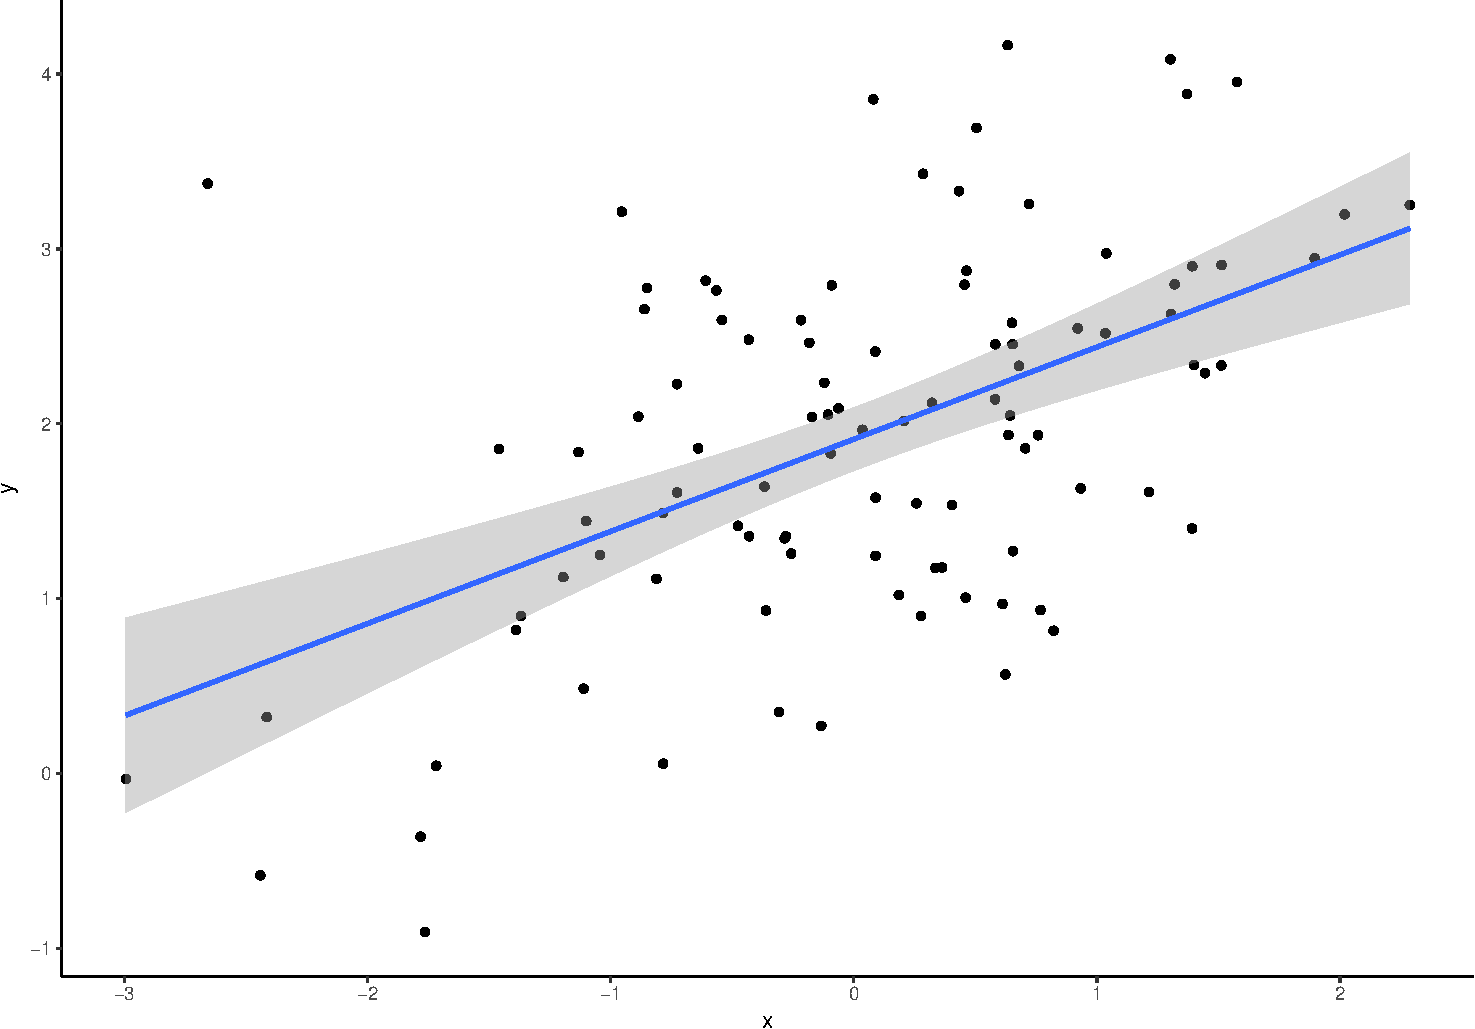
\includegraphics{slides_files/figure-beamer/unnamed-chunk-20-1.pdf}

\end{frame}

\begin{frame}[fragile]{RMarkdown: Example 4}
\protect\hypertarget{rmarkdown-example-4}{}

Likewise, tables from statistical models can be rendered and inserted
into the document.

\begin{verbatim}
```{r, echo=FALSE}
set.seed(42)
N <- 100
x <- rnorm(N)
Df <- data.frame(x = x, 
                 y = 0.0 + 0.25*x + rnorm(N))

M <- lm(y ~ x, data=Df)
pander(summary(M))
```
\end{verbatim}

\end{frame}

\begin{frame}{RMarkdown: Example 4 (rendered)}
\protect\hypertarget{rmarkdown-example-4-rendered}{}

\begin{longtable}[]{@{}ccccc@{}}
\toprule
\begin{minipage}[b]{0.21\columnwidth}\centering
~\strut
\end{minipage} & \begin{minipage}[b]{0.13\columnwidth}\centering
Estimate\strut
\end{minipage} & \begin{minipage}[b]{0.16\columnwidth}\centering
Std. Error\strut
\end{minipage} & \begin{minipage}[b]{0.12\columnwidth}\centering
t value\strut
\end{minipage} & \begin{minipage}[b]{0.12\columnwidth}\centering
Pr(\textgreater{}\textbar{}t\textbar{})\strut
\end{minipage}\tabularnewline
\midrule
\endhead
\begin{minipage}[t]{0.21\columnwidth}\centering
\textbf{(Intercept)}\strut
\end{minipage} & \begin{minipage}[t]{0.13\columnwidth}\centering
-0.088\strut
\end{minipage} & \begin{minipage}[t]{0.16\columnwidth}\centering
0.091\strut
\end{minipage} & \begin{minipage}[t]{0.12\columnwidth}\centering
-0.972\strut
\end{minipage} & \begin{minipage}[t]{0.12\columnwidth}\centering
0.333\strut
\end{minipage}\tabularnewline
\begin{minipage}[t]{0.21\columnwidth}\centering
\textbf{x}\strut
\end{minipage} & \begin{minipage}[t]{0.13\columnwidth}\centering
0.277\strut
\end{minipage} & \begin{minipage}[t]{0.16\columnwidth}\centering
0.088\strut
\end{minipage} & \begin{minipage}[t]{0.12\columnwidth}\centering
3.162\strut
\end{minipage} & \begin{minipage}[t]{0.12\columnwidth}\centering
0.002\strut
\end{minipage}\tabularnewline
\bottomrule
\end{longtable}

\begin{longtable}[]{@{}cccc@{}}
\caption{Fitting linear model: y \textasciitilde{} x}\tabularnewline
\toprule
\begin{minipage}[b]{0.18\columnwidth}\centering
Observations\strut
\end{minipage} & \begin{minipage}[b]{0.27\columnwidth}\centering
Residual Std. Error\strut
\end{minipage} & \begin{minipage}[b]{0.10\columnwidth}\centering
\(R^2\)\strut
\end{minipage} & \begin{minipage}[b]{0.20\columnwidth}\centering
Adjusted \(R^2\)\strut
\end{minipage}\tabularnewline
\midrule
\endfirsthead
\toprule
\begin{minipage}[b]{0.18\columnwidth}\centering
Observations\strut
\end{minipage} & \begin{minipage}[b]{0.27\columnwidth}\centering
Residual Std. Error\strut
\end{minipage} & \begin{minipage}[b]{0.10\columnwidth}\centering
\(R^2\)\strut
\end{minipage} & \begin{minipage}[b]{0.20\columnwidth}\centering
Adjusted \(R^2\)\strut
\end{minipage}\tabularnewline
\midrule
\endhead
\begin{minipage}[t]{0.18\columnwidth}\centering
100\strut
\end{minipage} & \begin{minipage}[t]{0.27\columnwidth}\centering
0.908\strut
\end{minipage} & \begin{minipage}[t]{0.10\columnwidth}\centering
0.093\strut
\end{minipage} & \begin{minipage}[t]{0.20\columnwidth}\centering
0.083\strut
\end{minipage}\tabularnewline
\bottomrule
\end{longtable}

\end{frame}

\begin{frame}[fragile]{RMarkdown: Example 5}
\protect\hypertarget{rmarkdown-example-5}{}

RMarkdown allows us to typeset mathematical equations, symbols, etc.,
just as we would do with \LaTeX.

\begin{verbatim}
```{r, echo=FALSE}
set.seed(42)
N <- 100
x <- rnorm(N)
Df <- data.frame(x = x, 
                 y = 0.0 + 0.25*x + rnorm(N))
M <- lm(y ~ x, data=Df)
```

The linear model is
$$
y_i = \alpha + \beta x_i + \epsilon_i, 
\quad \text{for $i \in 1 \ldots N$}.
$$

The $R^2$ value is `r round(mean(summary(M)$r.sq),2)`.
\end{verbatim}

\end{frame}

\begin{frame}{RMarkdown: Example 4 (rendered)}
\protect\hypertarget{rmarkdown-example-4-rendered-1}{}

The linear model is \[
y_i = \alpha + \beta x_i + \epsilon_i, 
\quad \text{for $i \in 1 \ldots N$}.
\]

The \(R^2\) value is 0.09.

\end{frame}

\begin{frame}[fragile]{RMarkdown, knitr, pandoc, papaja}
\protect\hypertarget{rmarkdown-knitr-pandoc-papaja}{}

\begin{itemize}
\item
  RMarkdown is basically a combination of a \emph{Markdown} document
  with embedded R code that is evaluated by
  \href{https://yihui.name/knitr/}{\texttt{knitr}}.
\item
  The resulting file is processed by pandoc to produce the desired
  output file type.
\item
  The three main output options are

  \begin{itemize}
  \tightlist
  \item
    pdf from \LaTeX
  \item
    MS Word
  \item
    HTML
  \end{itemize}
\item
  Tools like \href{https://github.com/crsh/papaja}{\texttt{papaja}}
  allow us to create APA formatted manuscripts from RMarkdown.
\item
  \texttt{knitr} can also be combined directly with \LaTeX, and this
  allows even more control of the final document.
\end{itemize}

\end{frame}

\begin{frame}{Jupyter notebooks}
\protect\hypertarget{jupyter-notebooks}{}

\begin{itemize}
\tightlist
\item
  Jupyter notebook are browser-based \emph{live} or \emph{dynamic}
  documents.
\item
  They are ideal for interactive work, prototype code development,
  visualization.
\item
  They generate rendered documents, e.g.~pdf via \LaTeX, html, etc, like
  RMarkdown.
\item
  Jupyter notebooks support multiple languages, but began as an
  extension of the IPython project, and Python is probably the most
  widely used language.
\end{itemize}

See demo available at \url{https://try.jupyter.org}

\end{frame}

\begin{frame}[fragile]{Git \& GitHub}
\protect\hypertarget{git-github}{}

\begin{itemize}
\tightlist
\item
  Git is version control software, initially developed for version
  control of the Linux operating system kernel.
\item
  It is now extremely widely used for almost all kinds of software
  development projects.
\item
  Git works on a decentralized system whereby a code-base can be
  \emph{cloned}, developed independently, and possible re-merged.
\item
  For collaborating on one project, two developers use a \emph{remote}
  host, clone it, develop locally, \emph{commit} and then \emph{push}
  back to and \emph{pull} from the remote host.
\item
  GitHub is one of the most widely used hosting sites (but there are
  others, e.g.~BitBucket; and running your own git hosting server is
  simple and inexpensive).
\item
  Git is designed for source code (i.e.~text files) management. Data and
  other “assets” can be attached to (rather than kept within) the
  repository using \texttt{git\ fat}, \texttt{git\ annex},
  \texttt{git\ lfs}, etc.
\end{itemize}

\end{frame}

\begin{frame}[fragile]{Git: Tiny tutorial}
\protect\hypertarget{git-tiny-tutorial}{}

\begin{itemize}
\tightlist
\item
  Start by cloning a remote repository:
\end{itemize}

\begin{Shaded}
\begin{Highlighting}[]
      \FunctionTok{git}\NormalTok{ clone https://github.com/yihui/knitr.git}
      \BuiltInTok{cd}\NormalTok{ knitr}
      \FunctionTok{git}\NormalTok{ log }\CommentTok{# Read all the commit logs}
\end{Highlighting}
\end{Shaded}

\begin{itemize}
\tightlist
\item
  Work as normal, i.e.~edit files, create new files, delete files.
\item
  You now \emph{stage} your changes, e.g.
\end{itemize}

\begin{Shaded}
\begin{Highlighting}[]
      \FunctionTok{git}\NormalTok{ add foo.file.1 foo.file.2 }\CommentTok{# for edits or new files}
      \FunctionTok{git}\NormalTok{ rm foo.file.3 }\CommentTok{# for removed files}
\end{Highlighting}
\end{Shaded}

\begin{itemize}
\tightlist
\item
  You then \emph{commit} these:
\end{itemize}

\begin{Shaded}
\begin{Highlighting}[]
      \FunctionTok{git}\NormalTok{ commit }\CommentTok{# Editor opens for your log msg}
\end{Highlighting}
\end{Shaded}

\end{frame}

\begin{frame}[fragile]{Git: Tiny tutorial (2)}
\protect\hypertarget{git-tiny-tutorial-2}{}

\begin{itemize}
\tightlist
\item
  Pull down any recent changes by others from the remote:
\end{itemize}

\begin{Shaded}
\begin{Highlighting}[]
      \FunctionTok{git}\NormalTok{ pull}
      \FunctionTok{git}\NormalTok{ log }\CommentTok{# If new changes, read their logs}
\end{Highlighting}
\end{Shaded}

\begin{itemize}
\tightlist
\item
  Now, push your own changes to the remote
\end{itemize}

\begin{Shaded}
\begin{Highlighting}[]
      \FunctionTok{git}\NormalTok{ push }\CommentTok{# requires permissions}
\end{Highlighting}
\end{Shaded}

\begin{itemize}
\tightlist
\item
  Undo changes:
\end{itemize}

\begin{Shaded}
\begin{Highlighting}[]
      \FunctionTok{git}\NormalTok{ reset a381f2f }\CommentTok{# move back "head"}
      \FunctionTok{git}\NormalTok{ revert a381f2f }\CommentTok{# applies new change to revert }
\end{Highlighting}
\end{Shaded}

\end{frame}

\begin{frame}{Conclusions}
\protect\hypertarget{conclusions}{}

\begin{itemize}
\tightlist
\item
  For open, transparent, and reproducible analysis, the code, data, and
  explanatory texts must be remain coupled.
\item
  RMarkdown (and knitr) and Jupyter notebooks are two complementary
  approaches to coupling data, code, and explanatory text.
\item
  Git \& GitHub allows us to manage, develop, and share these
  interdependent files.
\end{itemize}

\end{frame}

\end{document}
